\problemname{Dela ankor lika}
\noindent

Som en nådig härskare över POland vill du att alla dina invånare ska trivas. Det är därför djupt bekymrande
att två barn bråkar. Mer exakt bråkar de över $2N$ kodsportsankor som ligger
utplacerade på ett plan, och barnen grälar över hur många ankor var och en ska få.

För att lösa konflikten ska du skapa en spricka i marken - en rak linje som delar planet i två delar.
Sprickan måste placeras så att exakt $N$ ankor hamnar på vardera sida, vilket då leder till att vardera barn
får lika många ankor. Varje anka är utplacerad på en heltalskoordinat.

Eftersom du föredrar enkelhet och elegans kommer din spricka att vara en rät linje på formen $y=kx+m$,
där $k$ och $m$ får vara \textbf{decimaltal}. \\
Om det finns en linje som delar ankorna lika, skriv ut denna.\\ 
Skriv annars ut ''impossible''.

\section*{Indata}
Den första raden innehåller ett heltal $N$ ($1 \leq N \leq 10^5$), där $2N$ är det totala antalet ankor.

De följande $2N$ raderna beskriver ankornas positioner.
Varje rad innehåller två heltal $x_i, y_i$ ($0 \leq x_i, y_i \leq 10^6$), koordinaterna för den $i$:te ankan.
Alla ankor har olika positioner.

\section*{Utdata}
Om det är möjligt att dela ankorna lika, skriv ut två reella tal $k$ och $m$ ($-5 \cdot 10^9 \leq k, m \leq 5 \cdot 10^9$) som beskriver linjen $y = kx + m$.
$k$ och $m$ får innehålla som mest 50 tecken vardera. Domaren kommer att utföra alla beräkningar med $k$ och $m$ exakt. Notera att
ditt program kan avrunda $k$ och $m$ när de skrivs ut. \\
Svaret accepteras om linjen delar ankorna i två lika stora grupper. Om det finns flera lösningar kan du skriva ut vilken som helst.\\
Om en anka befinner sig exakt på linjen kommer det att räknas som att den är under linjen. 

Om det är omöjligt att dela ankorna lika, skriv ut ''impossible''.

\section*{Poängsättning}
Din lösning kommer att testas på en mängd testfallsgrupper.
För att få poäng för en grupp så måste du klara alla testfall i gruppen.

\noindent
\begin{tabular}{| l | l | p{12cm} |}
  \hline
  \textbf{Grupp} & \textbf{Poäng} & \textbf{Gränser} \\ \hline
  $1$    & $15$       & $N = 1$ \\ \hline
  $2$    & $15$       & $x_i = 0$ för alla ankor. \\ \hline
  $3$    & $15$       & $x_i \leq 1$ för alla ankor. \\ \hline
  $4$    & $15$       & $N = 2$ \\ \hline
  $5$    & $20$       & $N \leq 1000$ \\ \hline
  $6$    & $20$       & Inga ytterligare begränsningar. \\ \hline
\end{tabular}

\section*{Förklaring av exempelfall}
I varje av följande bilder har alla ankor ritats ut med svarta prickar. Sprickan som används i exempellösningen ritas ut som en röd linje.
Notera att det finns flera giltiga lösningar i alla dessa fallen.

\begin{centering}
  \begin{figure}[h]
      \centering
      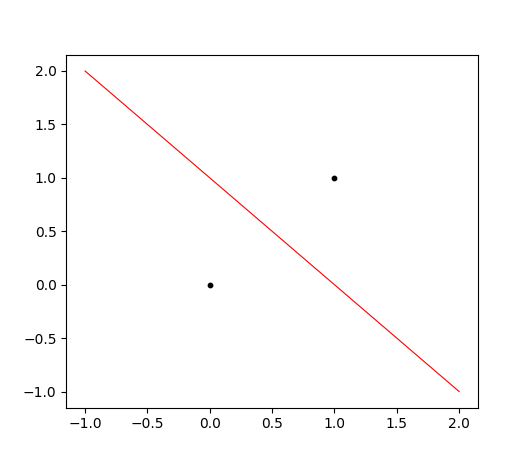
\includegraphics[width=0.3\textwidth]{sample1.png}
      \caption{Bilden föreställer det första exempelfallet.}
      \label{fig:enter-label}
  \end{figure}
\end{centering}

\begin{centering}
  \begin{figure}[h]
      \centering
      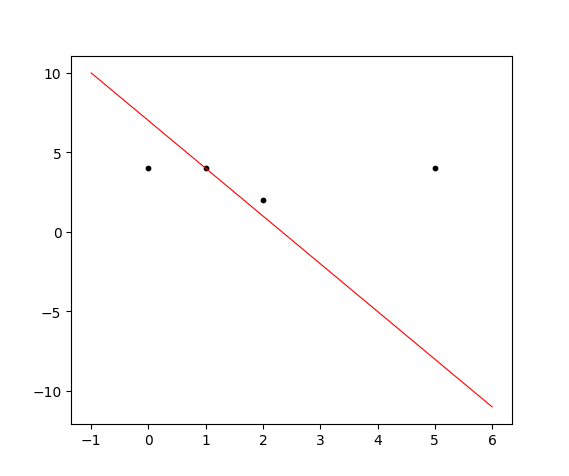
\includegraphics[width=0.3\textwidth]{sample2.png}
      \caption{Bilden föreställer det andra exempelfallet. Det är svårt att se, men den andra punkten
      är precis under linjen.}
      \label{fig:enter-label}
  \end{figure}
\end{centering}

\begin{centering}
  \begin{figure}[h]
      \centering
      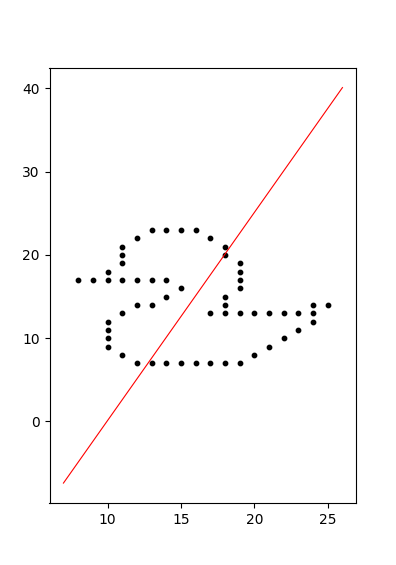
\includegraphics[width=0.3\textwidth]{sample3.png}
      \caption{Bilden föreställer det tredje exempelfallet.}
      \label{fig:enter-label}
  \end{figure}
\end{centering}